\documentclass[aspectratio=169,10pt]{beamer}
\usetheme{Madrid}
\usecolortheme{seahorse}
\usepackage{booktabs}
\usepackage{graphicx}
\usepackage{amsmath,amssymb}
\usepackage{xcolor}
\usepackage{tikz}
\usepackage{colortbl}
\usepackage{multirow}

\definecolor{vibblue}{RGB}{31,119,180}
\definecolor{viborange}{RGB}{255,127,14}
\definecolor{vibgreen}{RGB}{44,160,44}
\definecolor{vibred}{RGB}{214,39,40}

\setbeamertemplate{navigation symbols}{}
\setbeamertemplate{footline}[frame number]

% ────────────────────────────────────────────────────────────────────────────
\title[Multimodal VIB]{Variational Information Bottleneck\\for Audio-Visual Language Models}
\subtitle{Compression, Attention, and Modality Balance}
\author{Souleiman Sbais}
\date{\today}

\begin{document}

% ── Title ────────────────────────────────────────────────────────────────────
\begin{frame}
  \titlepage
\end{frame}

% ── Outline ──────────────────────────────────────────────────────────────────
\begin{frame}{Outline}
  \tableofcontents
\end{frame}

% ============================================================================
\section{Motivation and Setup}
% ============================================================================

\begin{frame}{Motivation}
  \begin{columns}
    \begin{column}{0.55\textwidth}
      \textbf{Problem}: Large multimodal LLMs receive thousands of raw encoder
      tokens. No compression $\Rightarrow$ no inductive bias toward informative
      content.

      \bigskip
      \textbf{Question}: Does a Variational Information Bottleneck (VIB) on
      audio/video tokens \ldots
      \begin{itemize}
        \item make the LLM \textbf{attend more locally}?
        \item change \textbf{how the LLM balances} modalities?
        \item open a path toward \textbf{prompt-conditioned routing}?
      \end{itemize}
    \end{column}
    \begin{column}{0.42\textwidth}
      \begin{block}{Base model}
        Qwen3-Omni 30B (frozen) \\
        + LoRA adapter \\
        + VIB on video tokens \\
        + VIB on audio tokens
      \end{block}
      \begin{block}{Task}
        Audio-Visual QA (AVQA) \\
        Audio-Visual Hallucination (AVHBench)
      \end{block}
    \end{column}
  \end{columns}
\end{frame}

\begin{frame}{Architecture Overview}
  \begin{center}
  \begin{tikzpicture}[node distance=1.2cm, every node/.style={font=\small}]
    \tikzstyle{box}=[rectangle,draw,rounded corners,minimum width=2.2cm,
                     minimum height=0.7cm,align=center]
    \tikzstyle{vib}=[box,fill=vibblue!20]
    \tikzstyle{llm}=[box,fill=vibgreen!20,minimum width=3cm]
    \tikzstyle{enc}=[box,fill=gray!15]

    \node[enc](venc){Video\\encoder};
    \node[enc,below=0.5cm of venc](aenc){Audio\\encoder};
    \node[vib,right=0.9cm of venc](vibv){Video VIB\\$z_v$};
    \node[vib,right=0.9cm of aenc](viba){Audio VIB\\$z_a$};
    \node[llm,right=1.8cm of vibv,yshift=-0.6cm](lm){LLM\\(frozen)};
    \node[box,right=0.9cm of lm](out){Answer};

    \draw[->](venc)--(vibv);
    \draw[->](aenc)--(viba);
    \draw[->](vibv)--(lm);
    \draw[->](viba)--(lm);
    \draw[->](lm)--(out);

    \node[above=0.1cm of vibv,font=\scriptsize,color=vibblue]{compress};
    \node[below=0.1cm of viba,font=\scriptsize,color=vibblue]{compress};
  \end{tikzpicture}
  \end{center}

  \medskip
  \begin{columns}
    \begin{column}{0.48\textwidth}
      \textbf{VIB objective}:
      \[\mathcal{L} = \underbrace{\text{NLL}}_{\text{task}} +
        \beta_v\,\text{KL}(q_v\|p) + \beta_a\,\text{KL}(q_a\|p)\]
    \end{column}
    \begin{column}{0.48\textwidth}
      \textbf{Training}: LoRA + VIB weights only.
      Backbone (30B) stays frozen. \\
      $\beta_v = \beta_a = 7{\times}10^{-6}$, 2000 steps on AVQA.
    \end{column}
  \end{columns}
\end{frame}

% ============================================================================
\section{Experiment 1: Attention Localization}
% ============================================================================

\begin{frame}{Experiment 1: Does the VIB Localize Attention?}
  \textbf{Setup}: From the same trained checkpoint, run two forwards per clip:
  \begin{itemize}
    \item \textbf{Without IB}: raw encoder tokens $\rightarrow$ LLM
    \item \textbf{With IB}: VIB-compressed tokens $\rightarrow$ LLM
  \end{itemize}

  \medskip
  Hook $q$-proj and $k$-proj in the last 8 decoder layers.
  Compute attention from the last prompt token over all visual token positions.

  \medskip
  \textbf{Localization metrics} (over visual token attention distribution $p$):
  \begin{columns}
    \begin{column}{0.48\textwidth}
      \[\text{norm-entropy} = \frac{H(p)}{\log N} \in [0,1]\]
      \centering\small Lower $\Rightarrow$ more localized
    \end{column}
    \begin{column}{0.48\textwidth}
      \[\text{top-5\%-mass} = \sum_{k \in \text{top-5\%}} p_k\]
      \centering\small Higher $\Rightarrow$ more localized
    \end{column}
  \end{columns}
\end{frame}

\begin{frame}{Attention Localization — Results (30 clips)}
  \begin{columns}
    \begin{column}{0.45\textwidth}
      \begin{block}{Aggregate over 30 clips}
        \renewcommand{\arraystretch}{1.3}
        \begin{tabular}{lcc}
          \toprule
          & Without IB & With IB \\
          \midrule
          norm-entropy & baseline & $-0.0043$ \\
          top-5\%-mass & baseline & $+0.0284$ \\
          \midrule
          IB wins $\downarrow$entropy & \multicolumn{2}{c}{\textbf{30/30}} \\
          IB wins $\uparrow$mass      & \multicolumn{2}{c}{\textbf{30/30}} \\
          \bottomrule
        \end{tabular}
      \end{block}
    \end{column}
    \begin{column}{0.52\textwidth}
      \includegraphics[width=\textwidth]{../meeting/ib_attention/0012y1s1bJI_000350_ib_compare.png}
    \end{column}
  \end{columns}

  \medskip
  \begin{alertblock}{Finding}
    A \emph{representational} VIB replicates the attention localization
    effect previously reported for \emph{attention} bottlenecks — on all 30
    clips without exception.
  \end{alertblock}
\end{frame}

% ============================================================================
\section{Experiment 2: Token-Level Analysis}
% ============================================================================

\begin{frame}{Experiment 2: What Does the LLM Actually Attend To?}
  \textbf{Setup}: For each clip, capture
  \begin{enumerate}
    \item Embeddings at visual/audio token positions at LLM layer 0 input
    \item Full-sequence attention from the last prompt token (all positions)
    \item Key norms for video, audio, and text tokens (last 8 layers)
  \end{enumerate}

  \medskip
  Run both conditions (raw / VIB) from the same checkpoint (10 clips).

  \medskip
  \begin{columns}
    \begin{column}{0.48\textwidth}
      \textbf{Video token count}: $\sim$2200 \\
      \textbf{Audio token count}: $\sim$130 \\
      \textbf{Ratio}: 17:1
    \end{column}
    \begin{column}{0.48\textwidth}
      \textbf{Naive expectation}: video $\approx$ 94\% of total attention \\
      \textbf{Observed}: video $\approx$ 83--91\%
    \end{column}
  \end{columns}
\end{frame}

\begin{frame}{Token Analysis — Key Results}
  \begin{columns}
    \begin{column}{0.52\textwidth}
      \textbf{Per-token attention (raw condition):}
      \renewcommand{\arraystretch}{1.3}
      \begin{tabular}{lccc}
        \toprule
        & Video & Audio & Text \\
        \midrule
        Per-token attn & $\sim$uniform & $1.5\times$ & $3\times$ \\
        Key norm & 11--12 & 12--14 & \textbf{15.6} \\
        \bottomrule
      \end{tabular}

      \bigskip
      \textbf{VIB effect on key norms:}
      \begin{tabular}{lcc}
        \toprule
        & Video & Audio \\
        \midrule
        $\Delta$ key norm & $+1$ & $\mathbf{-2}$ \\
        Embedding norm ratio & $2.2\times$ & $9.8\times$ \\
        Cosine similarity & 0.50 & \textbf{0.24} \\
        \bottomrule
      \end{tabular}
    \end{column}
    \begin{column}{0.45\textwidth}
      \begin{alertblock}{Finding 1}
        Video does \emph{not} dominate per-token attention.
        Audio receives more attention per token than video.
        Video dominates total mass purely by \textbf{token count (17:1)}.
      \end{alertblock}

      \medskip
      \begin{alertblock}{Finding 2}
        The VIB amplifies audio embeddings ($\times 9.8$ in norm) but
        \textbf{rotates them away} from their original direction
        (cos-sim = 0.24). After $k$-proj, audio keys become
        \emph{smaller}, suppressing audio's per-token advantage.
      \end{alertblock}
    \end{column}
  \end{columns}
\end{frame}

\begin{frame}{Why Audio Key Norms Drop}
  \begin{center}
  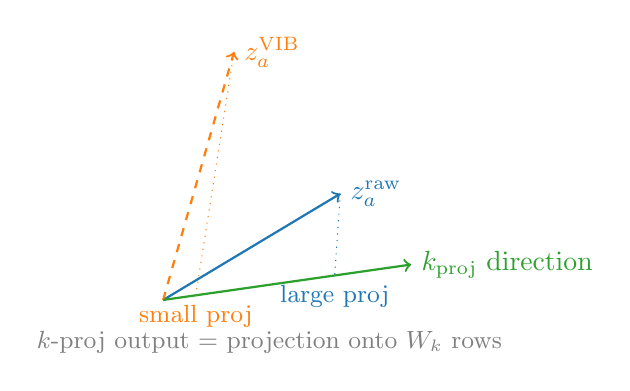
\begin{tikzpicture}[scale=0.9]
    % Raw audio
    \draw[->,thick,vibblue] (0,0) -- (2.5,1.5) node[right]{$z_a^{\text{raw}}$};
    % VIB audio (large norm, rotated)
    \draw[->,thick,viborange,dashed] (0,0) -- (1.0,3.5) node[right]{$z_a^{\text{VIB}}$};
    % k_proj axis
    \draw[->,thick,vibgreen] (0,0) -- (3.5,0.5) node[right]{$k_{\text{proj}}$ direction};
    % projections
    \draw[dotted,vibblue] (2.5,1.5) -- (2.42,0.34);
    \draw[dotted,viborange] (1.0,3.5) -- (0.46,0.066);
    \node[vibblue,below] at (2.42,0.34) {\small large proj};
    \node[viborange,below] at (0.46,0.066) {\small small proj};
    \node[gray] at (1.5,-0.6) {\small $k$-proj output = projection onto $W_k$ rows};
  \end{tikzpicture}
  \end{center}
  \begin{itemize}
    \item VIB output $z_a^{\text{VIB}}$ has large norm but wrong direction
    \item Its projection onto $k$-proj weight directions is \emph{smaller} than raw
    \item $\Rightarrow$ audio keys shrink $\Rightarrow$ audio receives less per-token attention
  \end{itemize}
\end{frame}

% ============================================================================
\section{Fixes: Balanced Audio Attention}
% ============================================================================

\begin{frame}{Fix 1 — Token-Count Equalization}
  \textbf{Observation}: $n_v \approx 2200$, $n_a \approx 130$, ratio $\approx 17$.

  \medskip
  \textbf{Fix}: After the VIB, scale audio tokens by $\sqrt{n_v / n_a} \approx 4.1$
  before splicing into $\texttt{inputs\_embeds}$:
  \[z_j = \bigl[\,z_v \;\big|\; \sqrt{\tfrac{n_v}{n_a}}\cdot z_a\,\bigr]\]

  \begin{columns}
    \begin{column}{0.55\textwidth}
      \begin{itemize}
        \item No training required — pure inference-time rescaling
        \item Makes audio's \textbf{total attention budget} equal to video's
        \item Equivalent to assigning equal prior weight to each modality
          regardless of how many tokens it uses
      \end{itemize}
    \end{column}
    \begin{column}{0.42\textwidth}
      \begin{block}{Expected effect}
        Audio total attn: $5\% \rightarrow \sim\!50\%$ \\
        (budget-equalised, not overcorrected\\
        since text still competes per-token)
      \end{block}
    \end{column}
  \end{columns}
\end{frame}

\begin{frame}{Fix 2 — Direction-Preservation Loss}
  \textbf{Observation}: VIB rotates audio tokens substantially (cos-sim = 0.24).
  This pushes $z_a^{\text{VIB}}$ away from the subspace that $k$-proj
  can strongly project onto.

  \medskip
  \textbf{Fix}: Add an auxiliary loss during VIB training:
  \[\mathcal{L}_{\text{dir}} = \lambda \cdot
    \bigl(1 - \cos\!\operatorname{sim}(z_a,\, z_a^{\text{raw}})\bigr)\]

  \begin{columns}
    \begin{column}{0.55\textwidth}
      \begin{itemize}
        \item Penalises directional rotation; allows magnitude change (compression)
        \item VIB can still compress (change norm) but must stay in the
          same directional subspace
        \item $k$-proj rows that responded to the raw audio still respond
          to the compressed audio
        \item $\lambda = 0.1$ (soft constraint)
      \end{itemize}
    \end{column}
    \begin{column}{0.42\textwidth}
      \begin{block}{Full training objective}
        $\mathcal{L} = \text{NLL} $\\
        $\quad + \beta_v \text{KL}_v + \beta_a \text{KL}_a $ \\
        $\quad + \lambda_{\text{dir}} \mathcal{L}_{\text{dir}}$ \\
        $\quad + \lambda_{\text{aux}} (\mathcal{L}_{\text{aux},v} + \mathcal{L}_{\text{aux},a})$
      \end{block}
    \end{column}
  \end{columns}
\end{frame}

% ============================================================================
\section{Extensions}
% ============================================================================

\begin{frame}{Extension 1 — Prompt-Conditioned Modality Gate}
  \textbf{Motivation}: ``What sound is being made?'' should weight audio
  more; ``What color is the object?'' should weight video more.

  \medskip
  \textbf{Architecture}:
  \begin{center}
  \begin{tikzpicture}[node distance=1.0cm, every node/.style={font=\small}]
    \tikzstyle{box}=[rectangle,draw,rounded corners,minimum width=2cm,
                     minimum height=0.6cm,align=center]
    \node[box,fill=gray!15](prompt){Prompt};
    \node[box,fill=vibblue!20,right=0.8cm of prompt](gate){Gate MLP\\$\rightarrow$ softmax};
    \node[box,fill=viborange!20,right=0.8cm of gate](p){$p_{\text{video}},p_{\text{audio}},p_{\text{text}}$};
    \node[box,fill=vibgreen!20,right=0.8cm of p](scale){Scale\\$z_v, z_a$};
    \draw[->](prompt)--(gate); \draw[->](gate)--(p); \draw[->](p)--(scale);
    \node[above=0.1cm of gate,font=\scriptsize]{mean-pool frozen embeddings};
    \node[below=0.1cm of p,font=\scriptsize]{centered: $M \cdot p$, uniform $= 1$};
  \end{tikzpicture}
  \end{center}

  \begin{columns}
    \begin{column}{0.48\textwidth}
      \begin{itemize}
        \item Gate zero-initialized $\Rightarrow$ untrained = identity
        \item Learns prompt-conditional modality routing end-to-end
        \item 1M additional parameters
      \end{itemize}
    \end{column}
    \begin{column}{0.48\textwidth}
      \begin{block}{Status}
        Trained 2000 steps on AVQA \\
        Final NLL loss: 0.364 \\
        Gate probe: pending
      \end{block}
    \end{column}
  \end{columns}
\end{frame}

\begin{frame}{Extension 2 — Perceive-then-Reason}
  \textbf{Motivation}: Give the VIB semantic context about what objects are
  present before compression.

  \medskip
  \textbf{Two-pass architecture}:
  \begin{enumerate}
    \item \textbf{Perception pass} (frozen): run the video through Qwen3-Omni
      with prompt ``List the main objects and scene.'' $\rightarrow$ text description
    \item \textbf{Reasoning pass}: VIB compresses video/audio, then
      \textbf{cross-modal attention} lets AV tokens attend to description embeddings
      before being spliced into the LLM
  \end{enumerate}

  \medskip
  \begin{columns}
    \begin{column}{0.55\textwidth}
      \textbf{Cross-modal attention} (trainable, zero-initialized):
      \[z_j \leftarrow z_j + \text{CrossAttn}(z_j,\, e_{\text{desc}})\]
      Queries = compressed AV tokens \\
      Keys/values = description embeddings (frozen)
    \end{column}
    \begin{column}{0.42\textwidth}
      \begin{block}{Hypothesis}
        Knowing ``car, traffic light, person''\\
        focuses VIB compression on those\\
        regions $\rightarrow$ sharper attention maps
      \end{block}
    \end{column}
  \end{columns}
\end{frame}

% ============================================================================
\section{Summary}
% ============================================================================

\begin{frame}{Summary of Findings}
  \renewcommand{\arraystretch}{1.4}
  \begin{tabular}{p{0.27\textwidth}p{0.65\textwidth}}
    \toprule
    \textbf{Experiment} & \textbf{Finding} \\
    \midrule
    IB attention & VIB makes LLM attention more spatially localized on
                   \textbf{30/30} clips ($\Delta$entropy $= -0.004$,
                   $\Delta$mass $= +0.028$) \\
    \midrule
    Token analysis & Video dominates total attention by \textbf{token count}
                    (17:1), not per-token preference. Audio receives more
                    attention per token than video. \\
    \midrule
    VIB key norms & VIB amplifies audio embeddings ($\times 9.8$) but
                   \textbf{rotates them} (cos-sim $= 0.24$), suppressing
                   audio key norms and inadvertently reducing audio's
                   per-token attention advantage. \\
    \midrule
    Balanced model & \textbf{Fix 1}: rescale audio by $\sqrt{n_v/n_a}$.
                     \textbf{Fix 2}: direction-preservation loss
                     $\lambda(1-\cos\operatorname{sim}(z_a, z_a^{\text{raw}}))$.
                     Training in progress. \\
    \bottomrule
  \end{tabular}
\end{frame}

\begin{frame}{Next Steps}
  \begin{enumerate}
    \item \textbf{Balanced model evaluation}: compare AVQA accuracy of
      balanced vs standard VIB. Do fixed audio key norms translate to better
      performance on audio-heavy questions?
    \item \textbf{Gate probe}: measure $p_{\text{video}}, p_{\text{audio}},
      p_{\text{text}}$ on held-out prompts. Does the gate assign higher
      audio weight to ``What sound is being made?'' vs ``What color is the car?''
    \item \textbf{Perceive-then-reason evaluation}: do description-informed
      attention maps concentrate on semantically relevant regions?
    \item \textbf{Rate-distortion curve}: vary $\beta$ from $10^{-6}$ to
      $10^{-5}$; plot AVQA accuracy vs mean KL to characterize the
      compression--performance tradeoff.
  \end{enumerate}
\end{frame}

\begin{frame}[standout]
  \centering
  \Large Thank you
\end{frame}

\end{document}
